\documentclass[french, a4paper,12pt, titlepage]{article}
\usepackage{babel}
\usepackage[utf8]{inputenc}
\usepackage[T1]{fontenc}
\usepackage{graphicx}
\usepackage{wrapfig}
\usepackage{layout}
\usepackage{amsmath}
\usepackage[top=2cm, bottom=2cm, left=2cm, right=2cm]{geometry}
\usepackage{parskip}
\DeclareUnicodeCharacter{00A0}{ }
\title{ {Systèmes et fonctions électroniques} \\ Devoir Maison 1}
\date{11 Novembre 2016}
\author{BELLA Jean-Paul \\ PIPEREAU Yohan}

\begin{document}
\maketitle

\newpage

\part*{\textbf{Partie Théorique}}


\paragraph{Question 1 : Ecrire la forme développer de \textbf{$s_1(t)$.} \\}
La forme développée du signal $s_1(t)$ en sortie du modulateur est
\begin{align*}
	s_{1}(t) & =  [ C + Db(t) ] a(t) \\
	& =  A cos(w_{p}t) [ C + DBcos(x_{m}t)]\\
	& =  AC [ cos(w_{p}t) +   \frac{m}{2}(cos(w_{p}t-w_{m}t) + cos(w_{p}t+w_{m}t) ]
\end{align*}
Soit \fbox{$ s_{1}(t)=  AC [ cos(w_{p}t) + \frac{m}{2}(cos(w_{p}t-w_{m}t) + cos(w_{p}t+w_{m}t) ]$} avec \fbox{$ m = \frac{DB}{C} $ }.\\


\paragraph{Question 2: Donner l'expression de $s_2(t)$. \\}
La forme développée de $s_2(t)$ en sortie du multiplieur est:
\begin{align*}
	s_{2}(t) & = s_{1}(t) a(t) \\
	&= A^{2} ( \frac{1+cos(2w_{p}(t)}{2} ) ( C + DBcos(w_{m}(t)) ) \\
	&=\frac{A^{2}C}{2} (1 + mcos(w_{m}t) + cos(2w_{p}t + \frac{m}{2} (cos (2w_{p}t-w_{m}t) + cos(2w_{p}t + w_{m}t) )
\end{align*}
Soit \fbox{$s_2(t)=\frac{A^{2}C}{2} (1 + mcos(w_{m}t) + cos(2w_{p}t + \frac{m}{2} (cos (2w_{p}t-w_{m}t) + cos(2w_{p}t + w_{m}t) )$}.

\paragraph{Question 3 : Comment choisir la pulsation de coupure du filtre passe-bas $w_{c}$ pour restituer fidelement le message? : \\ }
$w_{c}$  est la pulsation de coupure du filtre passe bas prenant en entrée  $s_{2}(t)$
et donnant en sortie le message qui était  $a(t)=A\cos(w_{p}t)$ .
Or,  $w_{m} \leq 2w_{p}-w_{m} \leq 2w_{p} \leq 2w_{p} + w_{m}$  où  $w_{m} \leq w_{p}$ . \\
Ainsi \fbox{ $w_{c} = w_{m}$ } \\

\newpage
\part*{\textbf{Simulation Labview}}

\begin{figure}[!h]
	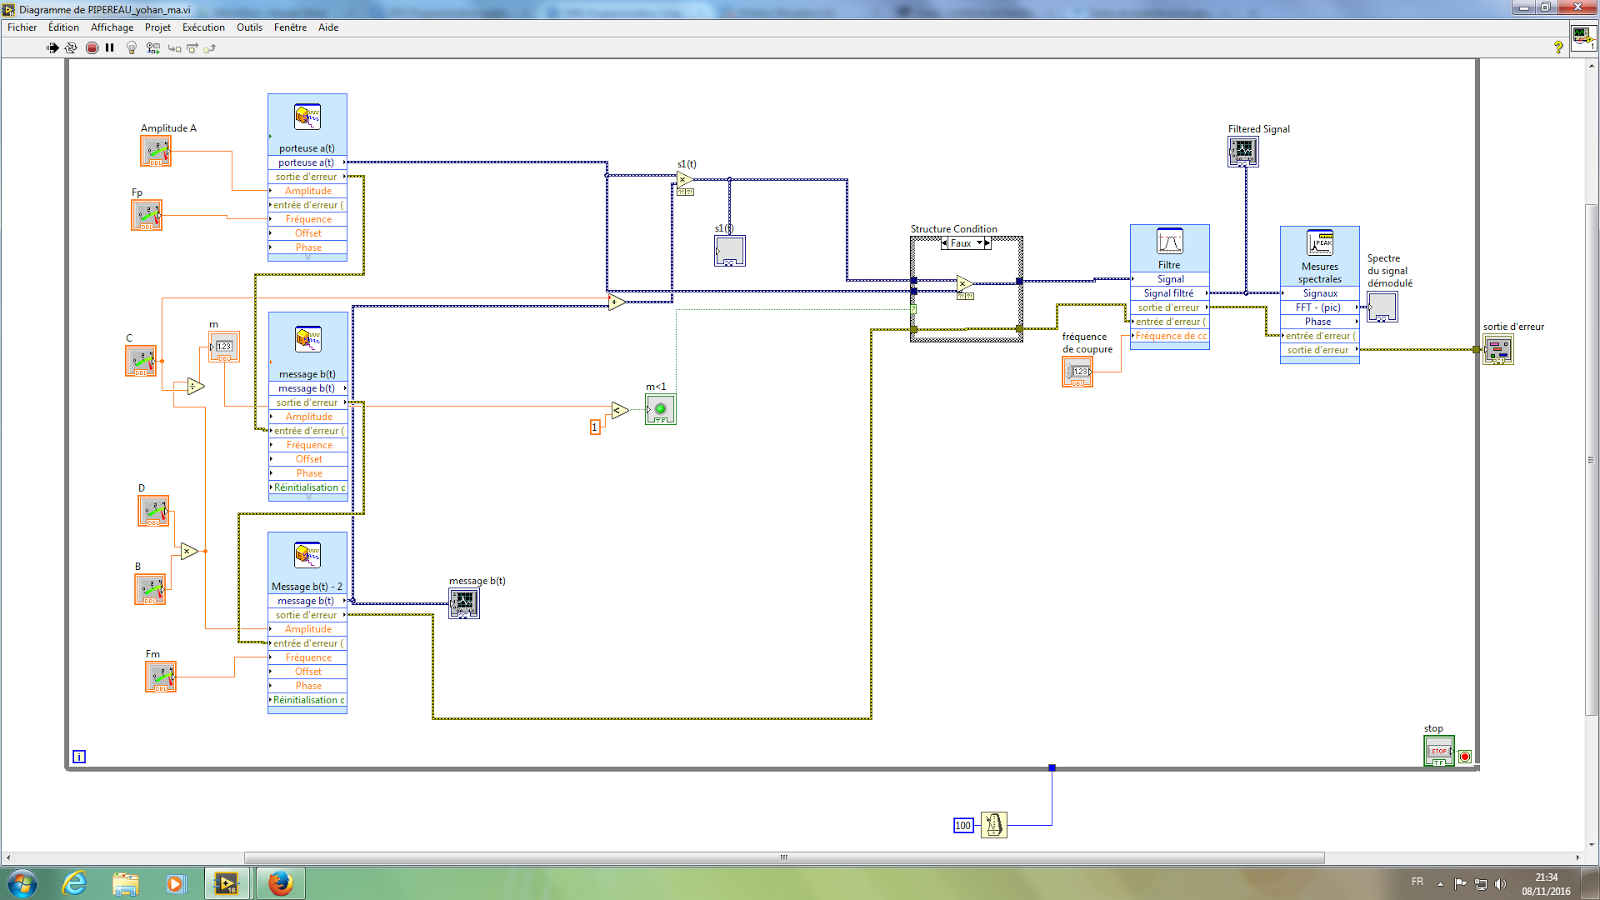
\includegraphics[width=\textwidth]{vuegenerale.png} \\
	\caption{Vue générale du programme Labview}
\end{figure}

	Nous avons mal compris l'énoncé et nous avons créé trois générateur au lieu de deux.
	Mais, le générateur inutile n'a aucune incidence dans le programme.

\begin{figure}[!h]
	\textbf{Question 4 : \\}
	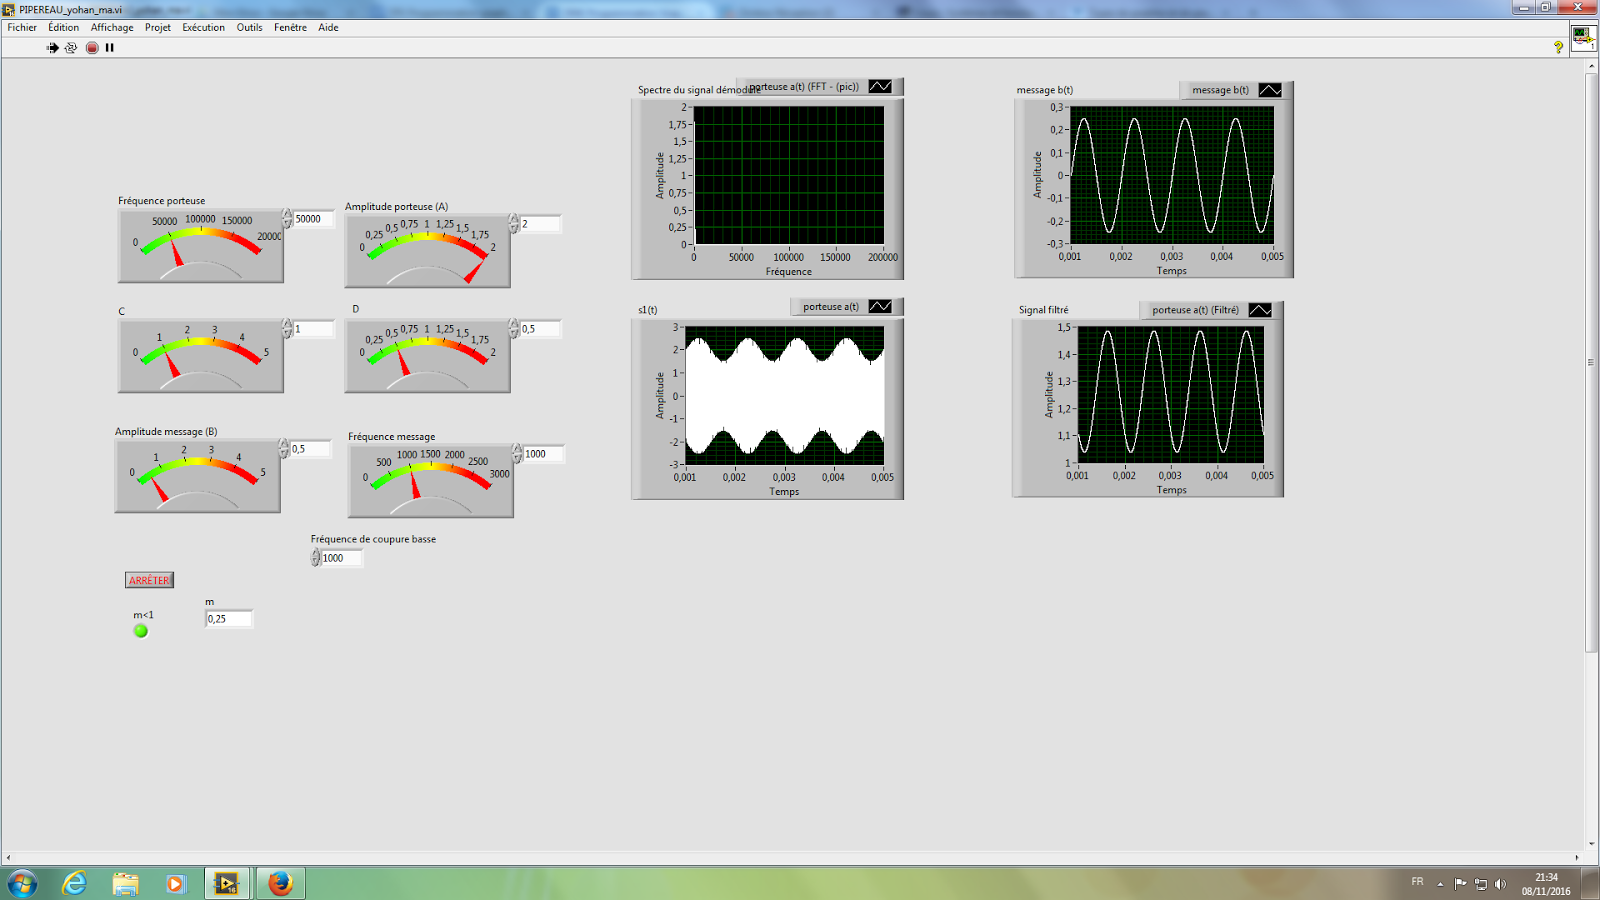
\includegraphics[width=\textwidth]{question4.png}
	\caption{ Test du vi avec  A = 2 ; B = 0,5 ; C = 1 ; D = 0.5 ; $f_p = 50kHz$ ; $f_m = 1kHz$}
\end{figure}

	Lors du test du vi avec les valeurs de la question 4, on a m=0.25.
	Le signal  $s_1(t)$ suit un signal sinusoïdal sous forme d’enveloppe (produit de sinusoïde).
	Le signal avant filtrage est une sinusoïde de fréquence $f_m$.

	La forme de l'onde émise est une sinusoïde d'harmonique égale à $f_m$, après modulation on observe une augmentation de l'amplitude
	et on constate également que la valeur moyenne a été décalée.

	Le décalage de la valeur moyenne peut s'expliquer par le fait que le filtre passe-bas conserve la valeur moyenne et que celle-ci a donc
	subi les modifications liées au multiplexage et démultiplexage.
	Le spectre possède un pic à 5000 Hz (et quelques pics autour) indiquant la présence de l'harmonique du signal du message que
	l’on retrouve après démodulation.

\begin{figure}[!h]
	\textbf{Question 5 : \\ }
	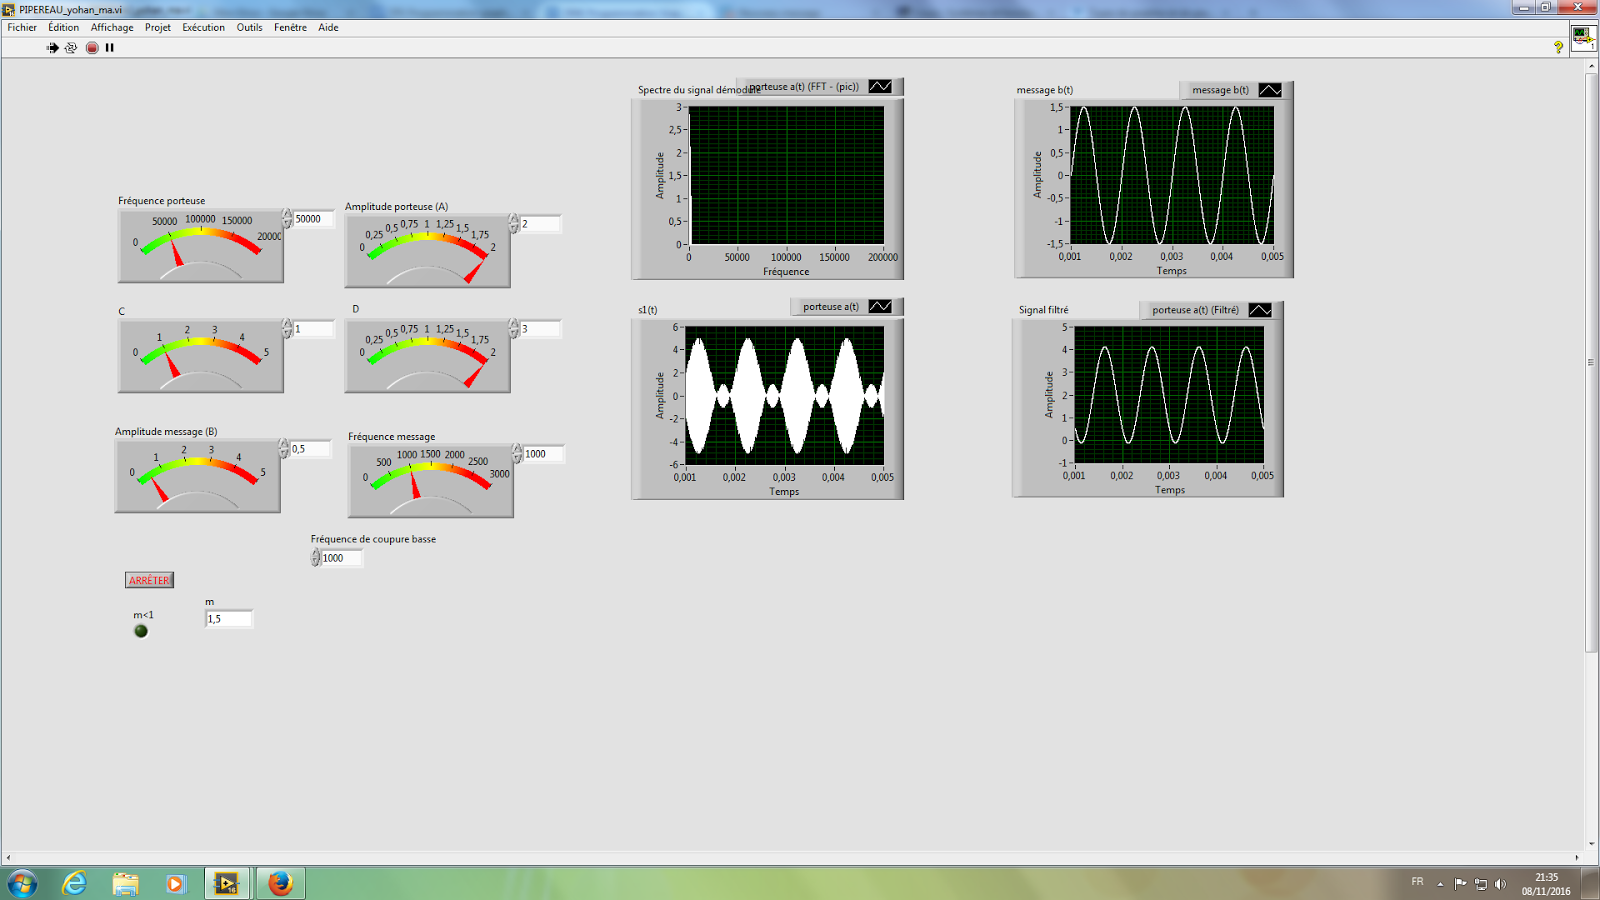
\includegraphics[width=\textwidth]{question5.png}
	\caption{Test du vi avec  A = 2 ; B = 0,5 ; C = 1 ; D = 3 ; $f_p = 50kHz$ ; $f_m = 1kHz$}
\end{figure}

Lors du test du vi avec les valeurs de la question 5, on a m=1.5.

L'harmonique reste la même.

La forme de l'onde émise est une sinusoïde d'harmonique égale à $f_m$, après modulation on observe une augmentation de l'amplitude
et on constate également que la valeur moyenne a été décalée.
L'explication a déjà fournie précédemment.

\newpage

\begin{figure}[!h]
	\textbf{Question 6 : \\ }
	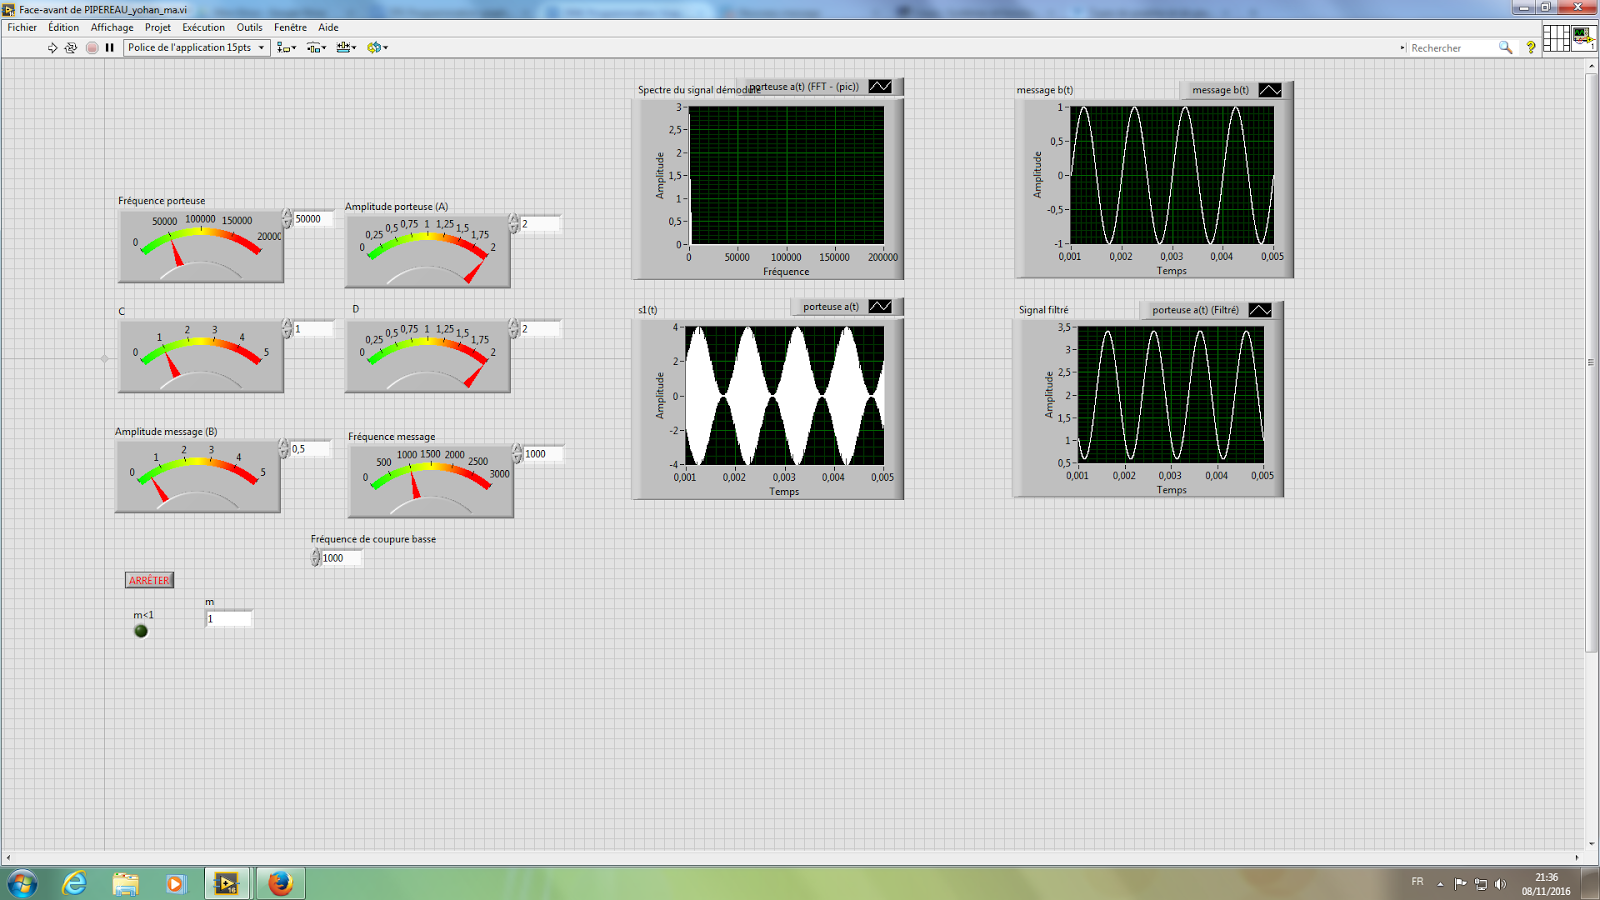
\includegraphics[width=\textwidth]{question6.png}
	\caption{ Test du vi avec A = 2; B = 0,5 ; C = 1 ; D = 2 ; $f_p = 50kHz$ ; $f_m = 1kHz$  }
\end{figure}

Lors du test du vi avec les valeurs de la question 6, on a m=1.

La forme de l'onde émise est une sinusoïde d'harmonique égale à $f_m$, après modulation on observe une augmentation de l'amplitude
et on constate également que la valeur moyenne a été décalée.
L'explication a déjà été fournie précédemment.

\begin{figure}[!h]
	\textbf{Question 7 : Que deviennent les formes d’onde pour un message de forme carré, d’amplitude B=0,25V les autres valeurs restant inchangées? \\}
	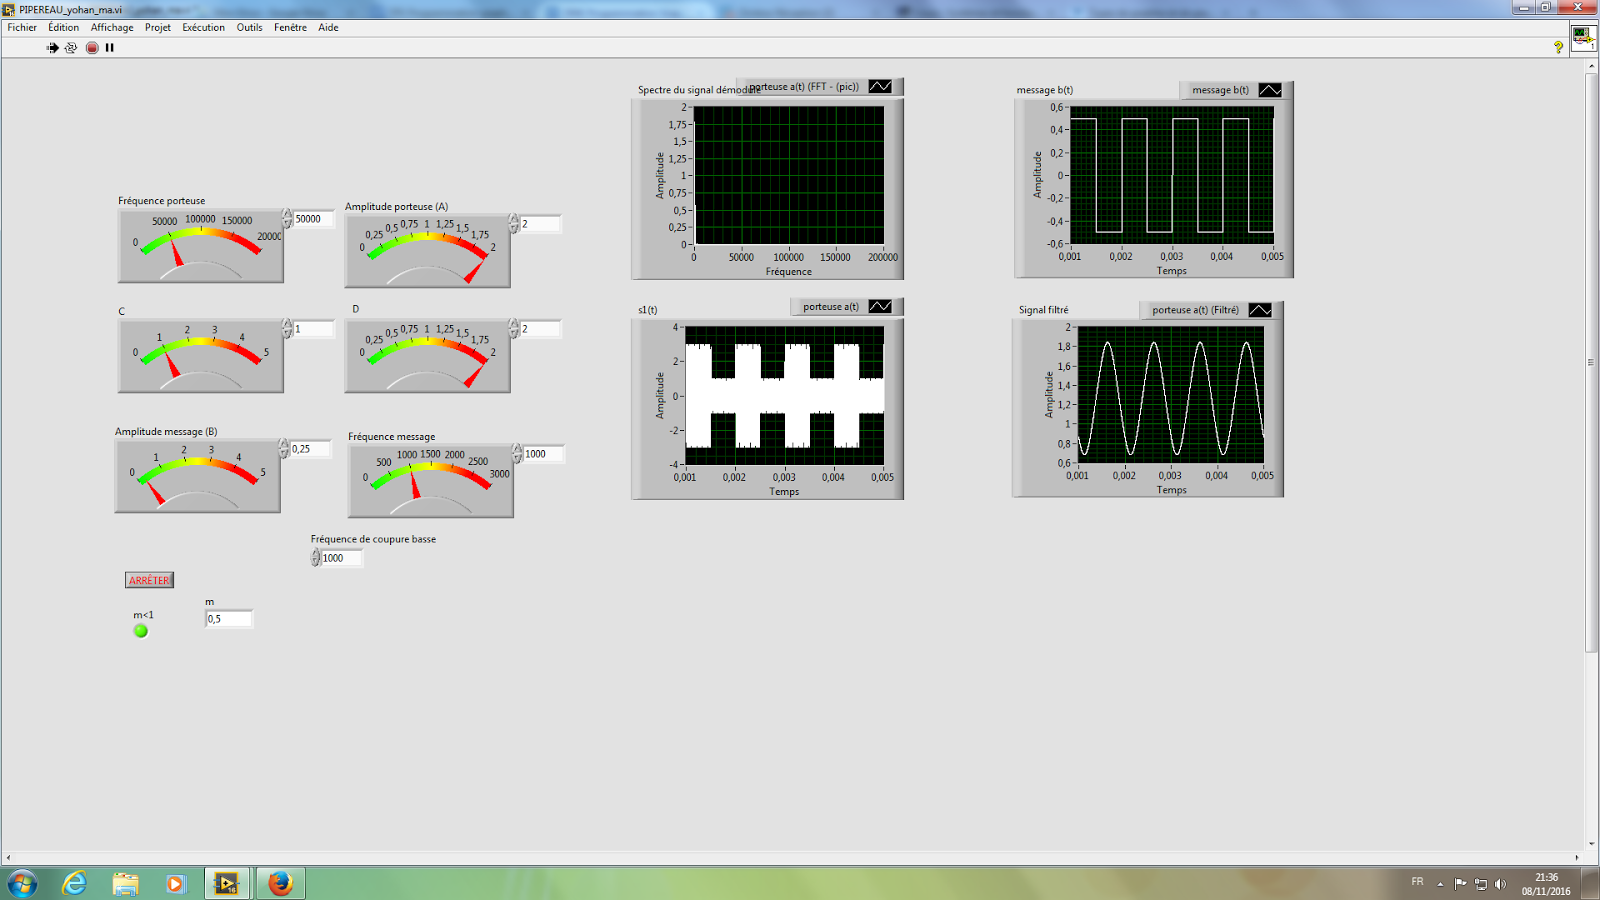
\includegraphics[width=\textwidth]{question7.png}
	\caption{	Test du vi avec des ondes carrées d'amplitudes B=0.25V }
\end{figure}

Lors de l'émission d'un message crénau, on obtient après modulation une onde sinusoïdale de fréquence égale à celle de l'harmonique du signal d'entrée.
On peut expliquer ce phénomène par le filtrage des fréquences supérieures à $w_c$ par le filtre passe bas. Ce qui conserve uniquement l'harmonique du signal
et filtre les hautes fréquences responsables de la forme du signal.
\end{document}
